

\section{Data preparation}

%TODO add reference
The COMPAS dataset used in this study is publicly available through ProPublica's GitHub repository. This repository contains the dataset and other assets used by ProPublica to investigate the biases present in the COMPAS risk assessment tool.

The file chosen for this analysis is \textbf{\texttt{compas-scores-two-years.csv}}, as it provides the cleanest and most relevant data for general recidivism prediction. This CSV file contains the key data required for our study, including several attributes related to demographics, criminal history, COMPAS risk scores, and the two-year recidivism outcomes that are important for exploring the predictive capabilities and the ethical implications of machine learning models in the context of recidivism prediction. 

The dataset includes important information about individuals. Following an initial analysis, a list of the key fields in the dataset is below.

\begin{itemize}
	
	\item Personal Information, includes attributes such as \textbf{\texttt{age}}, \textbf{\texttt{race}}, \textbf{\texttt{age\_category}}, etc.
	
	\item Case and Event-Related Details are the fields prefixed with \textbf{\texttt{c\_}} that provide a timeline and details of a person's interactions with the criminal justice system.
	
	\item Violence Risk Assessment are the fields prefixed with \textbf{\texttt{v\_}} and are associated with the violence risk assessment in COMPAS. This dimension predicts violent recidivism risk.
	
	\item Case-Level Details for Violent Recidivism are the fields prefixed with \textbf{\texttt{vr\_}}. These fields provide additional details specific to violent recidivism events.
	
	\item Juvenile Criminal Record are the fields prefixed with \textbf{\texttt{juv\_}}. These fields capture information about an individual's juvenile criminal record, which is a key predictor of future adult criminal behaviour.
	
	\item Previous Charges and Severity can be deduced from fields such as \textbf{\texttt{priors\_count}} and \textbf{\texttt{juv\_}} fields.
	
	\item Additional fields, including \textbf{\texttt{r\_charge\_}}, \textbf{\texttt{r\_offense\_}}, \textbf{\texttt{vr\_}} fields, \textbf{\texttt{c\_charge\_degree}}, and \textbf{\texttt{c\_charge\_desc}}, provide a broader perspective on criminal history and severity.
	
	
	\item Two-Year Recidivism, or the \textbf{\texttt{two\_year\_recid}} field in the COMPAS dataset, indicates whether an individual reoffended (recidivated) within two years of their initial assessment or release. This field is critical for evaluating the predictive accuracy of the COMPAS risk assessment tool.
	
	\item Decile Score is a standardized risk score in the COMPAS dataset. It categorizes an individual's likelihood of recidivism into ten equal groups (deciles) where 1 is the lowest risk, and 10 is the highest risk. Each decile represents approximately 10\% of the sample when applied to a norm group.
	
\end{itemize}

%Suppose that we observe the following data:

%\begin{table}[!ht]
%	\centering
%	\begin{tabular}{|l|l|}
%		\hline
%		Field & Value \\ \hline
%		\textbf{\texttt{priors\_count}} & 5 \\ \hline
%		\textbf{\texttt{juv\_felony\_count}} & 2 \\ \hline
%		\textbf{\texttt{juv\_misdemeanor\_count}} & 3 \\ \hline
%		\textbf{\texttt{r\_charge\_degree}} & Felony \\ \hline
%	\end{tabular}
%\end{table}

%We can interpret this as an individual who has five total prior charges, including:

%\begin{itemize}
%	\item 2 juvenile felonies
%	\item 3 juvenile misdemeanours
%	\item The severity of previous charges includes felonies (\textbf{\texttt{r\_charge\_degree}}).
%\end{itemize}


\subsection{Preparing the data for further analysis and training}

Before we can perform any analysis or apply machine learning techniques, it is important to pre-process and prepare the dataset so that we can handle missing values, encode categorical features, and split the data into training, testing, and validation sets. This step will produce a clean dataset for building accurate and unbiased models. The following steps outline the procedures to prepare the dataset for further analysis and training.


\subsection{Initial look at data and missing values handling}

The dataset has 7214 instances over 53 columns. The COMPAS system risk factor is the field  \textbf{\texttt{decile\_score}}, but the dataset also contains information about whether or not the person recidivised through the label \textbf{\texttt{two\_year\_recid}}. 

The first step in this data analysis step was  removing the features irrelevant to this exercise or with over 50\% missing records. We removed all the COMPAS-administrative labels and additional recidivism information apart from \textbf{\texttt{two\_year\_recid}}, narrowing the dataset to 17 fields.

The difference between \textbf{\texttt{c\_jail\_in}} and \textbf{\texttt{c\_jail\_out}} was calculated into a new field, \textbf{\texttt{days\_in\_jail}} and the difference between \textbf{\texttt{in\_custody}} and \textbf{\texttt{out\_custody}}, in a new field, \textbf{\texttt{days\_in\_custody}}. We subsequently removed the features containing date information from the dataset, together with \textbf{\texttt{days\_in\_custody}}, as it contained no information. At this stage, the dataset contains thirteen features: eight numerical, four categorical, and one descriptive. It also contains two labels, decile\_score, which we will treat as the leading label in this exercise and \textbf{\texttt{two\_year\_recid}}, which we are keeping to compare the prediction power of our models to the original one.


\subsection{Imputation of missing data}

While examining the resultant dataset, we noticed that \textbf{\texttt{days\_b\_screening\_arrest}} has  6907 values that are not null. Whilst it is possible to eliminate the rows that contain the null values at this stage, we replaced the missing values using a KNN imputation technique by grouping the numeric values of this dataset so that we can calculate the missing values. We checked this process by plotting the distribution of \textbf{\texttt{days\_b\_screening\_arrest}} before and after imputation to see if any variations occurred.

\begin{figure}[H]
	\centering
	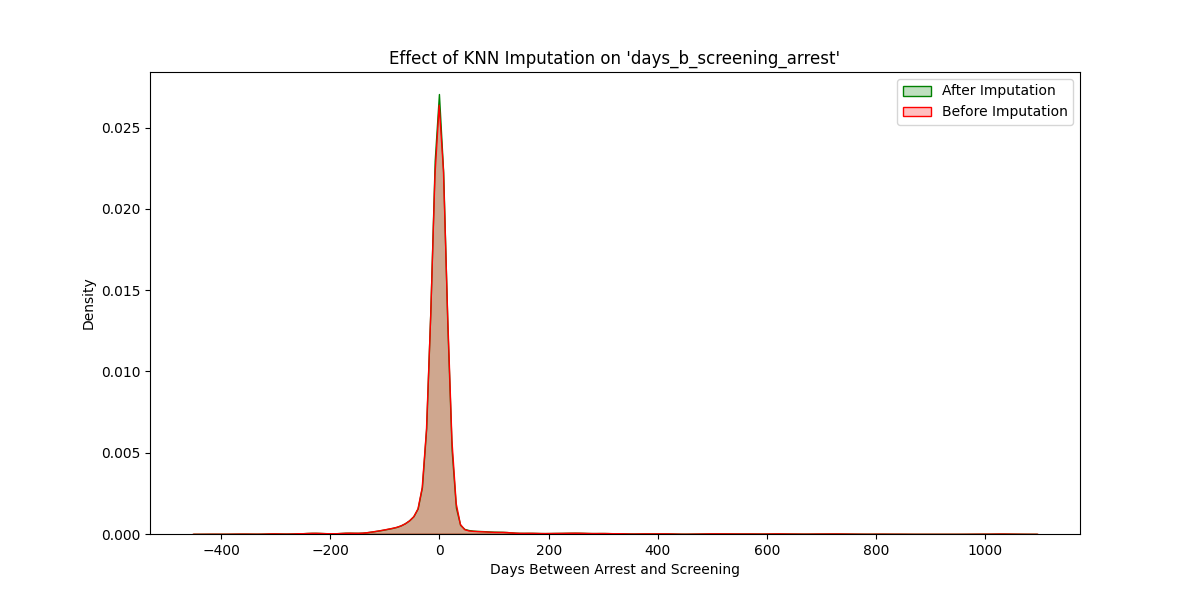
\includegraphics[width=0.9\linewidth]{img/imputation}
	\caption[Distribution \textbf{\texttt{days\_b\_screening\_arrest}} of before and after KNN imputation]{}
	\label{fig:imputation}
\end{figure}

At this stage, the dataset contains four categorical features that need encoding for machine learning algorithms. This section will focus on converting them into a numerical format using two encoding techniques. The categorical features and their values are listed below:

\begin{table}[!ht]
	\centering
	\begin{tabular}{|l|l|l|}
		\hline
		Feature & Description & Unique Values \\ \hline\hline
		\textbf{\texttt{sex}} & Gender of the individual & \shortstack{Male\\Female} \\ \hline
		\textbf{\texttt{race}} & Race of the individual & \shortstack[l]{African-American\\Caucasian\\Hispanic\\Asian\\Native American\\Other} \\ \hline
		\textbf{\texttt{age\_cat}} & Age category & \shortstack[l]{Less than 25\\25 - 45\\Greater than 45} \\ \hline
		\textbf{\texttt{c\_charge\_degree}} & \shortstack{Degree of the\\criminal charge} & \shortstack[l]{F (Felony)\\M (Misdemeanor)} \\ \hline
	\end{tabular}
\end{table}

The following transformations are applied:

\begin{itemize}[]
	\item One-Hot Encoding on \textbf{\texttt{sex}}, \textbf{\texttt{race}}, and \textbf{\texttt{c\_charge\_degree}}, transforming them into binary columns.
	\item Ordinal Encoding on \textbf{\texttt{age\_cat}}. This encoding technique was preferred over one-hot in this case as it preserves order, thus respecting the inherent ranking of the category.
\end{itemize}

The original categorical columns were retained in the dataset for future use in the analysis steps. 

\subsection{Splitting the data into train, test and dev}

A stratified shuffle split technique is preferred to create the train, test, and dev datasets whilst ensuring that the splits are proportional by \textbf{\texttt{race}}. In the first split, 80\% Train and 20\% Test are created, whilst in the Second split, The 20\% Test is further divided into 10\% Test and 10\% Dev.


\section{Data exploration and visualisation}

Here we will examine the dataset in more detail to understand the patterns, distributions, and relationships. In this exercise, we will use more of the visual tools available through several Python libraries to identify potential biases, explore correlations between variables, and uncover insights that may influence the outcomes of predictive models. 

\subsection {Demographic analysis}

We begin this analysis by segmenting the dataset based by race and gender.





\begin{figure}[H]
	\centering
	% First image
	\begin{subfigure}[b]{0.45\linewidth}
		\centering
		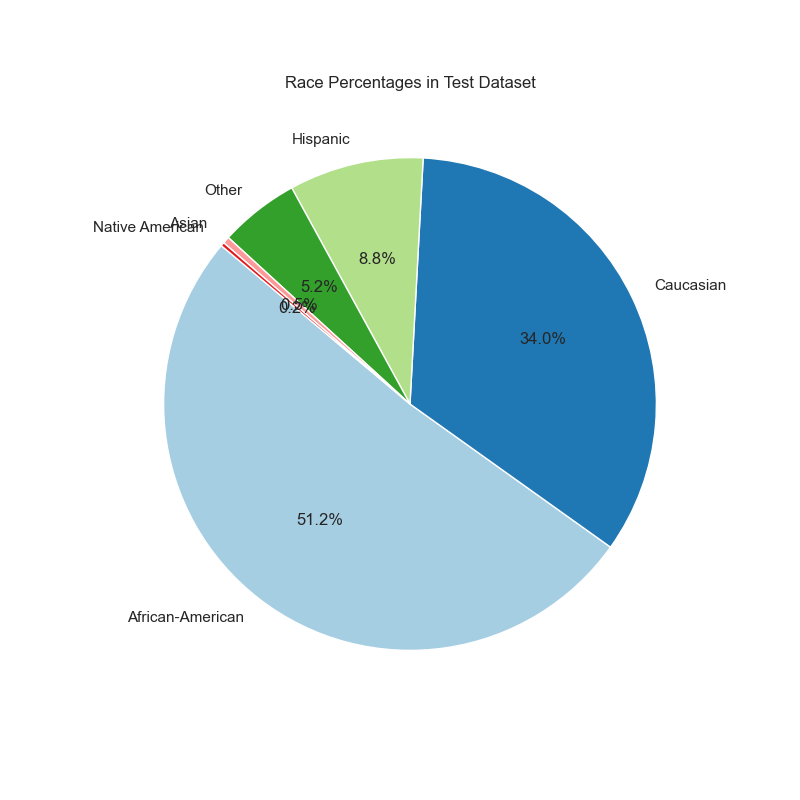
\includegraphics[width=\linewidth]{img/race_percentages_pie.png}
	\end{subfigure}
	\hfill
	% Second image
	\begin{subfigure}[b]{0.45\linewidth}
		\centering
		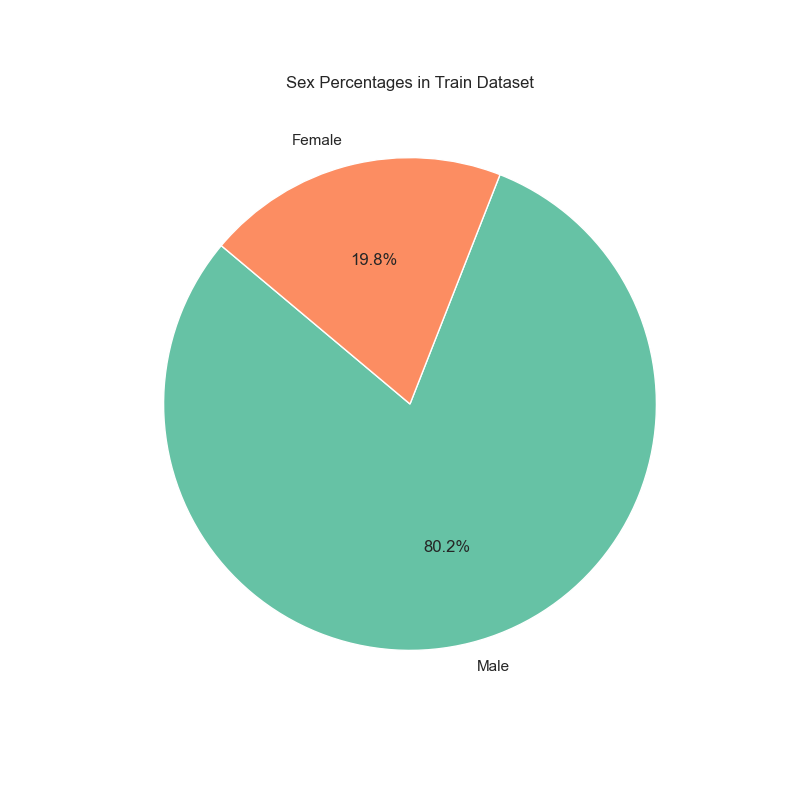
\includegraphics[width=\linewidth]{img/sex_percentages_pie.png}
	\end{subfigure}
	\caption{Race and Sex breakdown for the dataset.}
	\label{fig:race-sex-breakdown}
\end{figure}


%% First image
%\begin{figure}
%	\centering
%	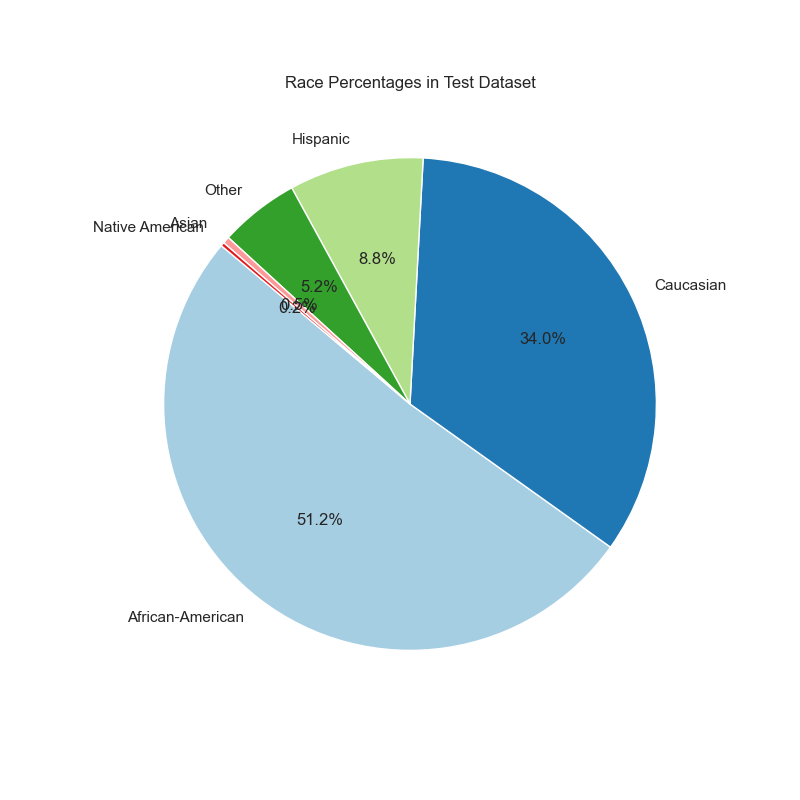
\includegraphics[width=0.7\linewidth]{img/race_percentages_pie.png}
%	\caption{Caption for the first image}
%	\label{fig:image1}
%\end{figure}
%\hfill
%% Second image
%\begin{figure}
%	\centering
%	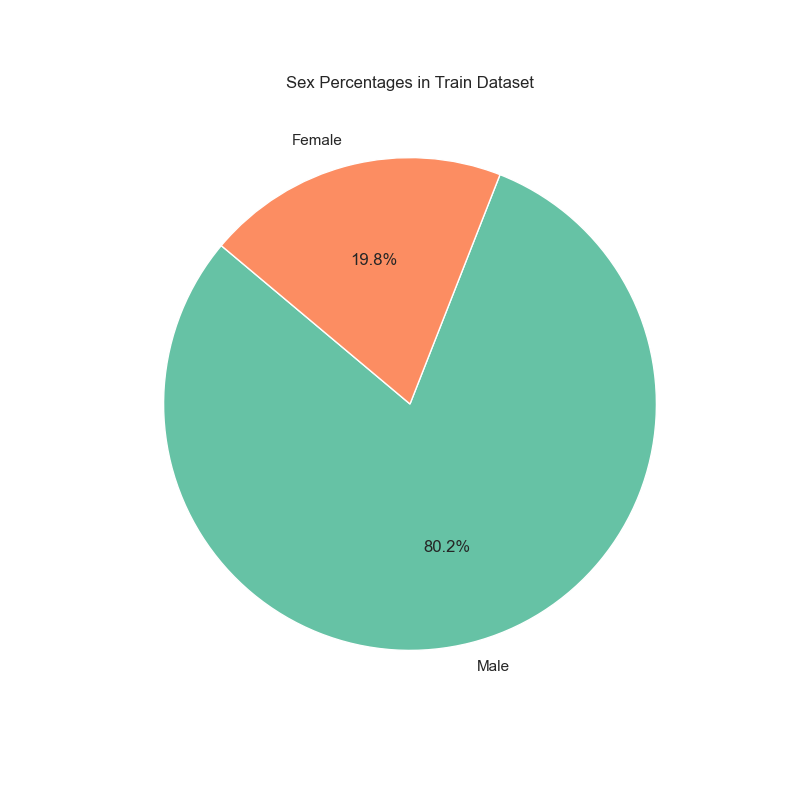
\includegraphics[width=0.7\linewidth]{img/sex_percentages_pie.png}
%	\caption{Caption for the second image}
%	\label{fig:image2}
%\end{figure}


By examining the racial composition of the dataset, we observe the following:

\begin{itemize}
	\item Over half of the test dataset is composed of African-American individuals, suggesting that the dataset may be imbalanced, with a disproportionate representation of one racial group.
	\item Asians and Native Americans each makeup only 0.2\% of the dataset; this underrepresentation might raise some concerns as it may lead to challenges in statistical analysis or machine learning models. Such concerns include the lack of reliability or significance for these groups due to insufficient data.
\end{itemize}

Figure \ref{fig:race-sex-breakdown} also shows our dataset's male/female split, with females comprising only 19.8\%. It is, therefore, evident that the female group is underrepresented, which can lead to biased models as models may overfit male patterns and underperform on females and misleading conclusions as insights derived might generalise poorly for the female subgroup.


\subsection{Age distribution analysis}


We used a boxplot to illustrate the age patterns across racial groups, helping to identify central values, spread, and any anomalies.

\begin{figure}[H]
	\centering
	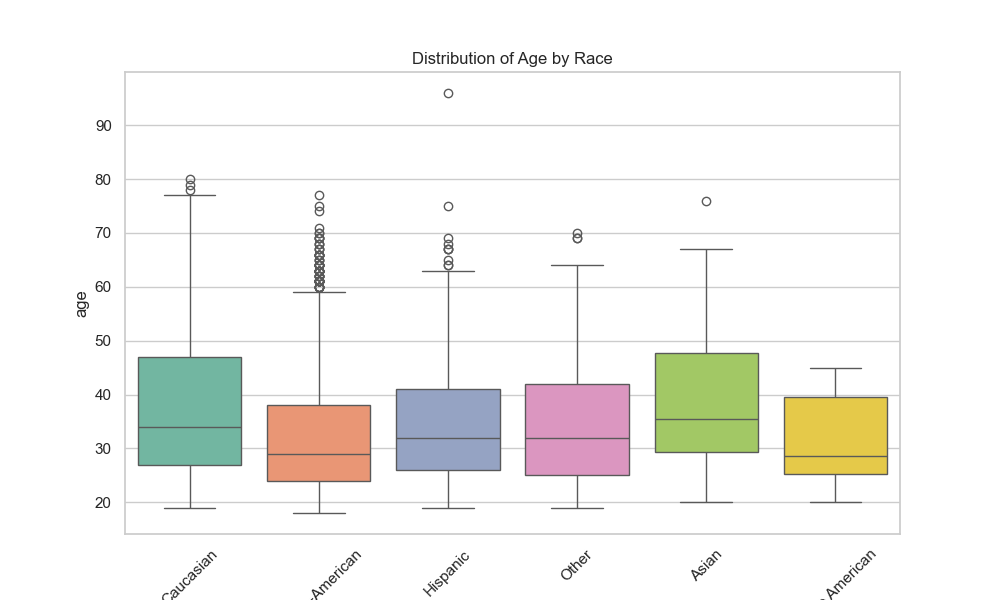
\includegraphics[width=0.9	\linewidth]{img/age_by_race_boxplot}
	\caption{}
	\label{fig:age-by-race-boxplot}
\end{figure}



\begin{table}[H]
	\centering
	\begin{tabular}{|l|l|p{4cm}|}
		\hline
		Race & Median Age & Distribution Description \\ \hline \hline
		African-American & $\approx$30 years & Concentrated in the 20–40 range, with a relatively narrow spread. We notice outliers above 60 years,  indicating fewer older individuals. \\ \hline
		Caucasian & $\approx$40 years & Broader age range, from 20 to 70+ years. We notice more older individuals (upper outliers), making this group appear older on average. \\ \hline
		Hispanic & $\approx$30–35 years & Moderately broad spread, with most individuals between 20 and 50 years. \\ \hline
		Asian & $\approx$30 years & Narrow distribution, concentrated between 25 and 40 years. No outliers. \\ \hline
		Native American & $\approx$33 years & Very tight distribution, with all ages clustered closely around the median (little variability). It is important to note that this group accounts for a tiny portion of the population. \\ \hline
		Other & $\approx$35–40 years & Similar to Caucasians but with slightly fewer older individuals. The IQR shows a widespread. \\ \hline
	\end{tabular}
\end{table}



\subsection{Analysing distributions}


Next, we plotted the distributions of all the features in our dataset; this is depicted in Figure \ref{fig:distribution-plots} . From these histograms, we notice 
\begin{itemize}
	\item The age distribution shows a right-skewed pattern, with most individuals falling in the younger age ranges (20–40 years).
	
	\item There is a significant over-representation of certain racial groups, particularly African Americans, which could indicate potential biases in the dataset's sampling.
	
	\item Most individuals have zero juvenile felony counts, zero juvenile misdemeanour counts, and no recorded "other" juvenile offences, with each distribution rapidly declining for higher counts.
	
	\item A large proportion of individuals have a low number of prior offences, but there is a long tail indicating some individuals have a significant number of priors.
	
	\item Most individuals have relatively short jail durations, with a few experiencing significantly longer durations.
	
	\item The distribution of days between screening and arrest is clustered around zero, with few extreme outliers on both ends.
	
	\item The decile scores appear relatively evenly distributed, but slight patterns suggest clustering at specific score levels (e.g., lower decile scores are slightly more frequent).
	
	\item Two-year recidivism plot shows a near-equal distribution, indicating a balanced dataset for recidivism outcomes.
\end{itemize}


\begin{figure}[H]
	\centering
	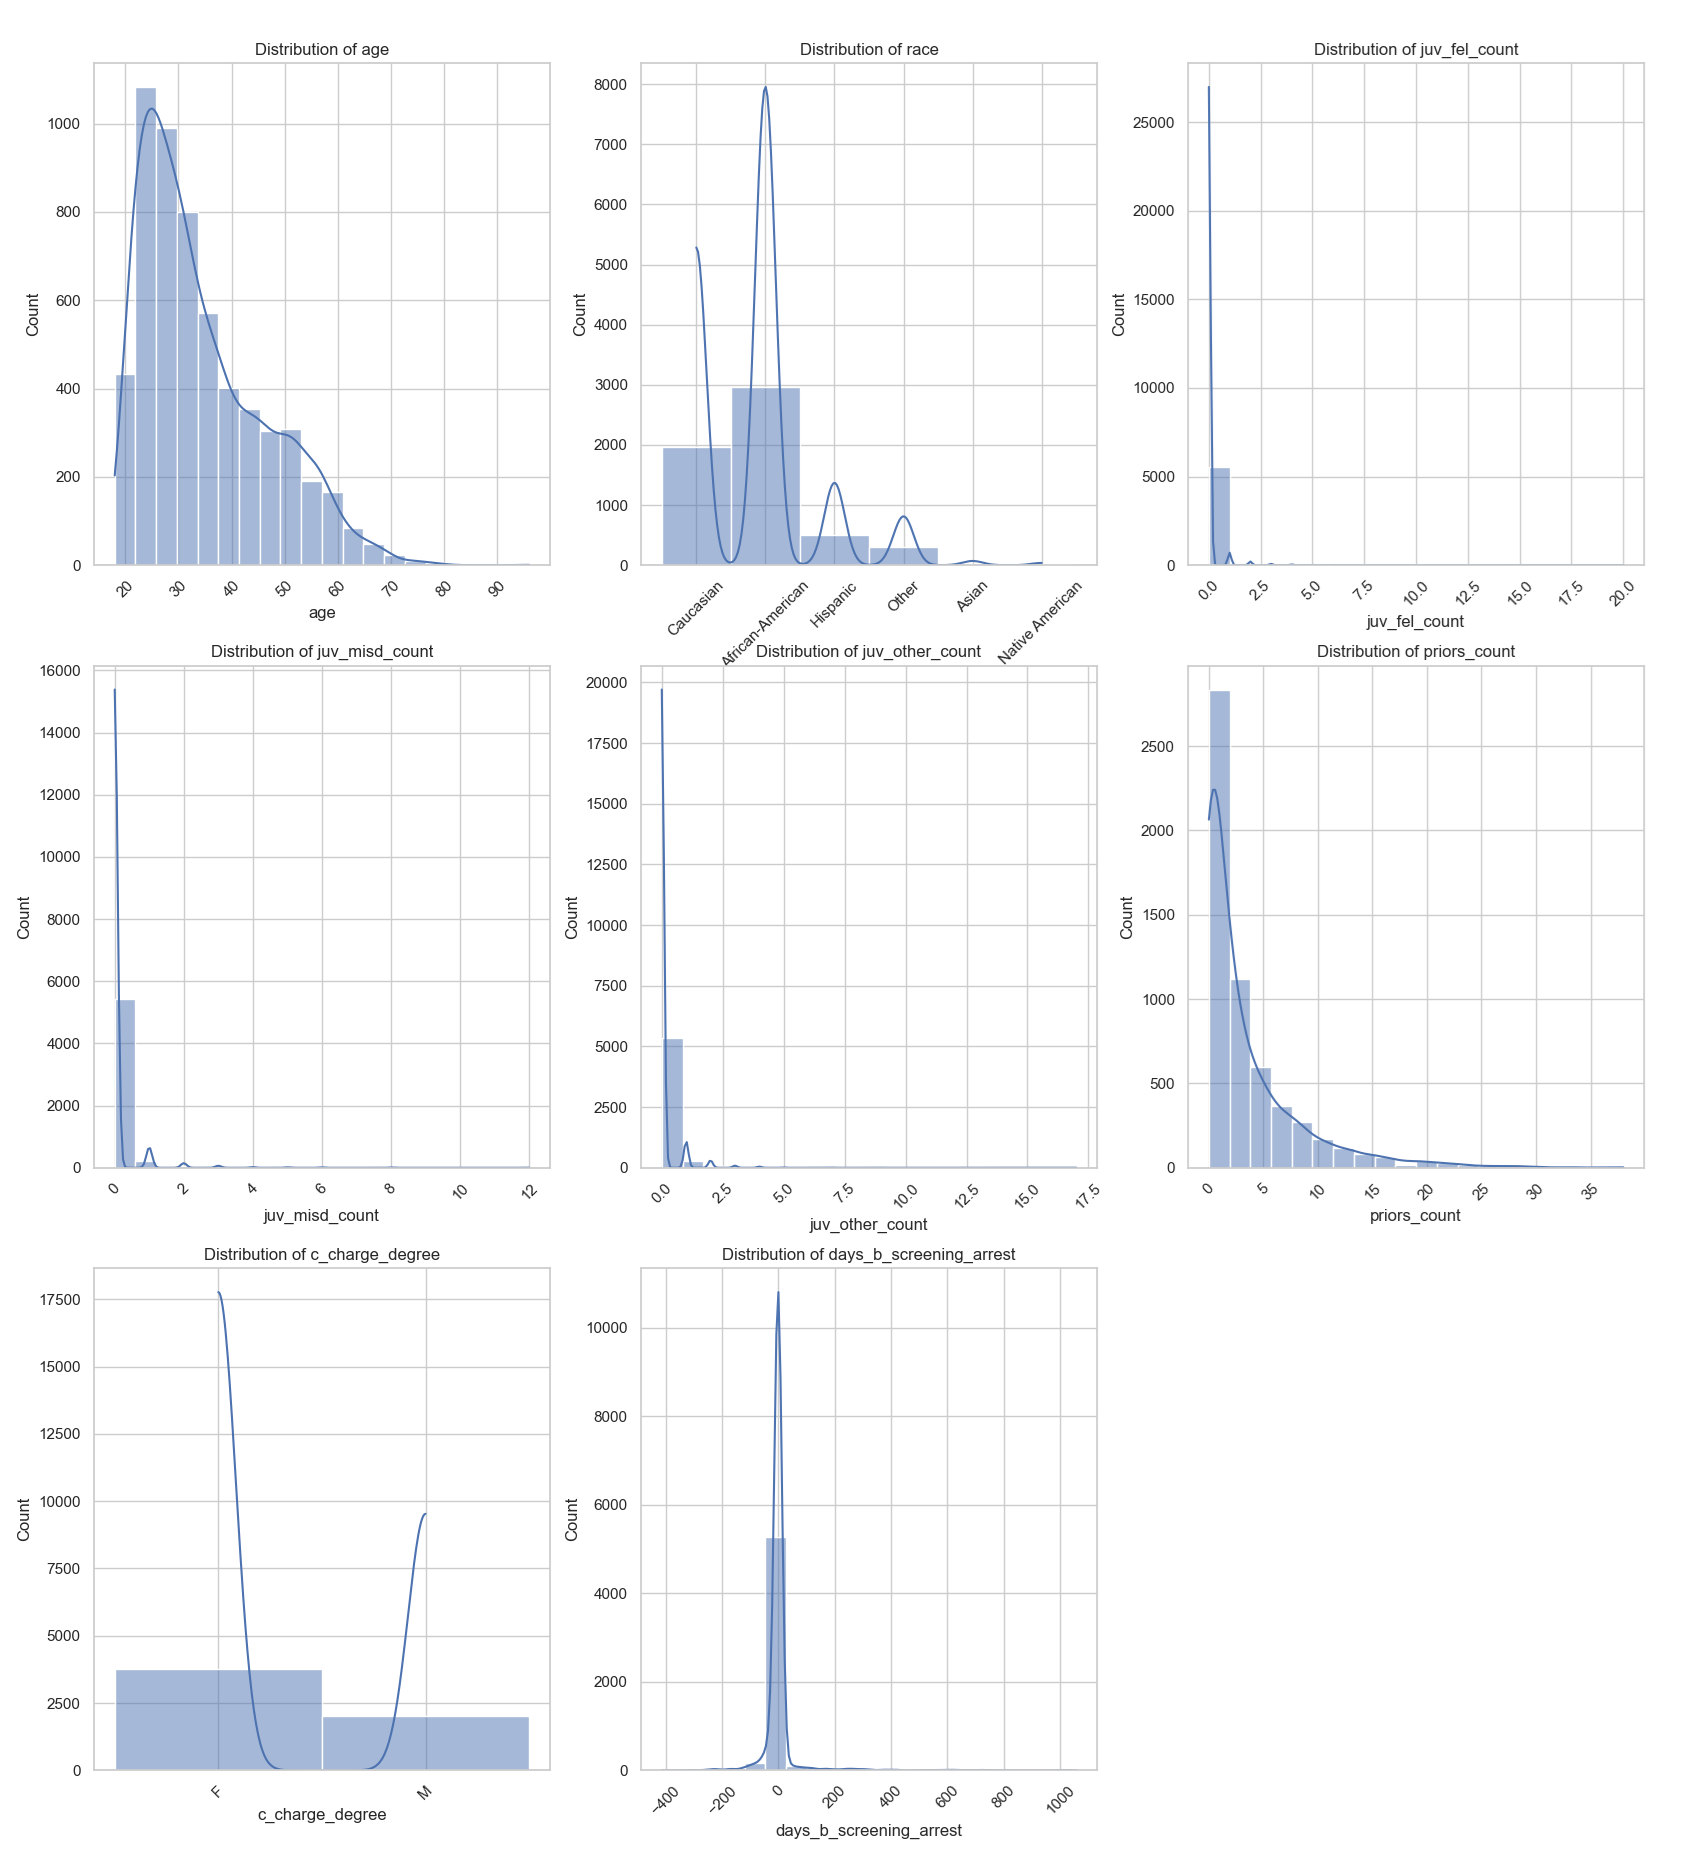
\includegraphics[width=0.9\linewidth]{img/distribution-plots}
	\caption{}
	\label{fig:distribution-plots}
\end{figure}


\subsection{Correlation analysis}

The correlation matrix heatmap shown in Figure \ref{fig:correlationmatrixheatmap} was created to gather more insights and pinpoint the areas of high correlation. This plot raises a number of interesting observations, namely:

\begin{figure}[!h]
	\centering
	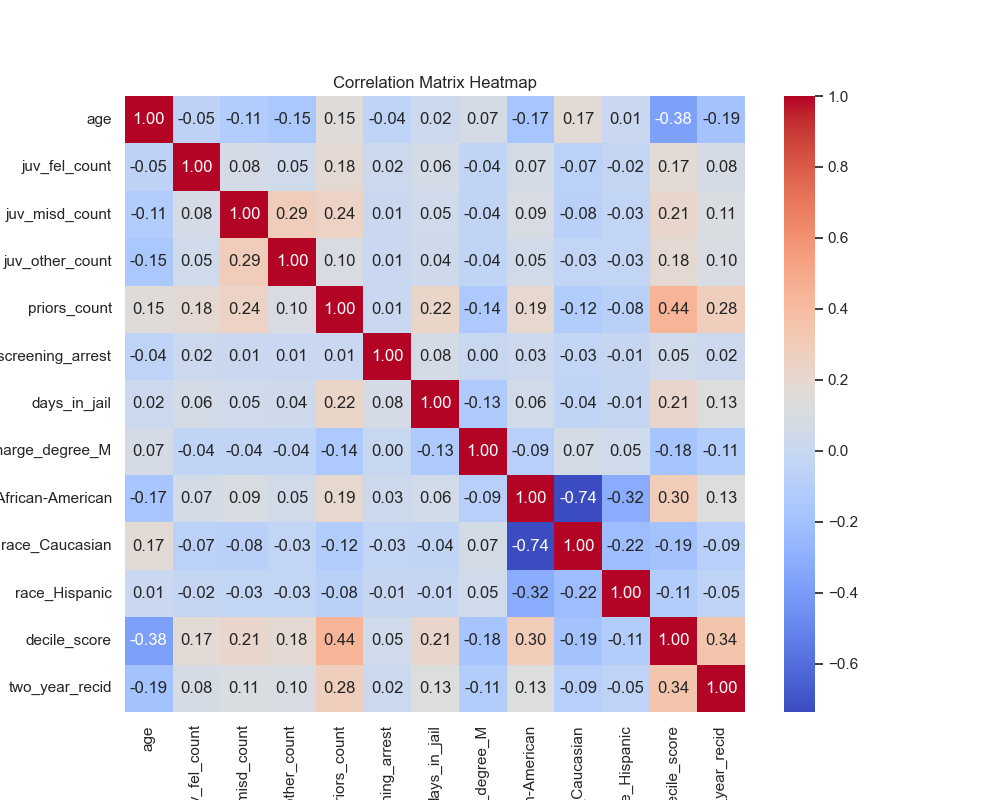
\includegraphics[width=0.7\linewidth]{img/correlation_matrix_heatmap}
	\caption{}
	\label{fig:correlationmatrixheatmap}
\end{figure}


\begin{itemize}
	\item Individuals with more prior offences tend to have higher risk scores, as prior criminal behaviour is a key factor in risk assessment models. The number of prior offences also correlates positively with recidivism; individuals with more prior offences tend to re-offend more often.
	
	\item Older individuals tend to have lower risk scores, suggesting that age may be inversely related to the risk of recidivism, with younger individuals being assessed as higher risk. In addition, older individuals are also less likely to recidivate, supporting this general trend.
	
	\item Individuals with higher risk scores are likelier to recidivate within two years, suggesting that the risk score (\textbf{\texttt{decile\_score}}) is predictive to a certain extent of recidivism.
	
	\item A correlation of 0.30 indicates that being African-American is moderately associated with higher decile scores, raising potential concerns about racial bias in the scoring system. At the same time, Caucasian individuals correlate -0.19 and, therefore, are less likely to receive higher risk scores.
	
	\item The time spent in jail has only a small positive relationship with the likelihood of re-offending within two years
	
	\item  Juvenile felony, misdemeanour, and other counts are positively correlated, indicating that individuals with one type of juvenile record will often have other types.
\end{itemize}

Figure \ref{fig:pairplot} is a pair plot created to substantiate these observations further to show the relationships among the selected numerical features, with the recidivism outcome (\textbf{\texttt{two\_year\_recid}}) as the hue.

\begin{figure}
	\centering
	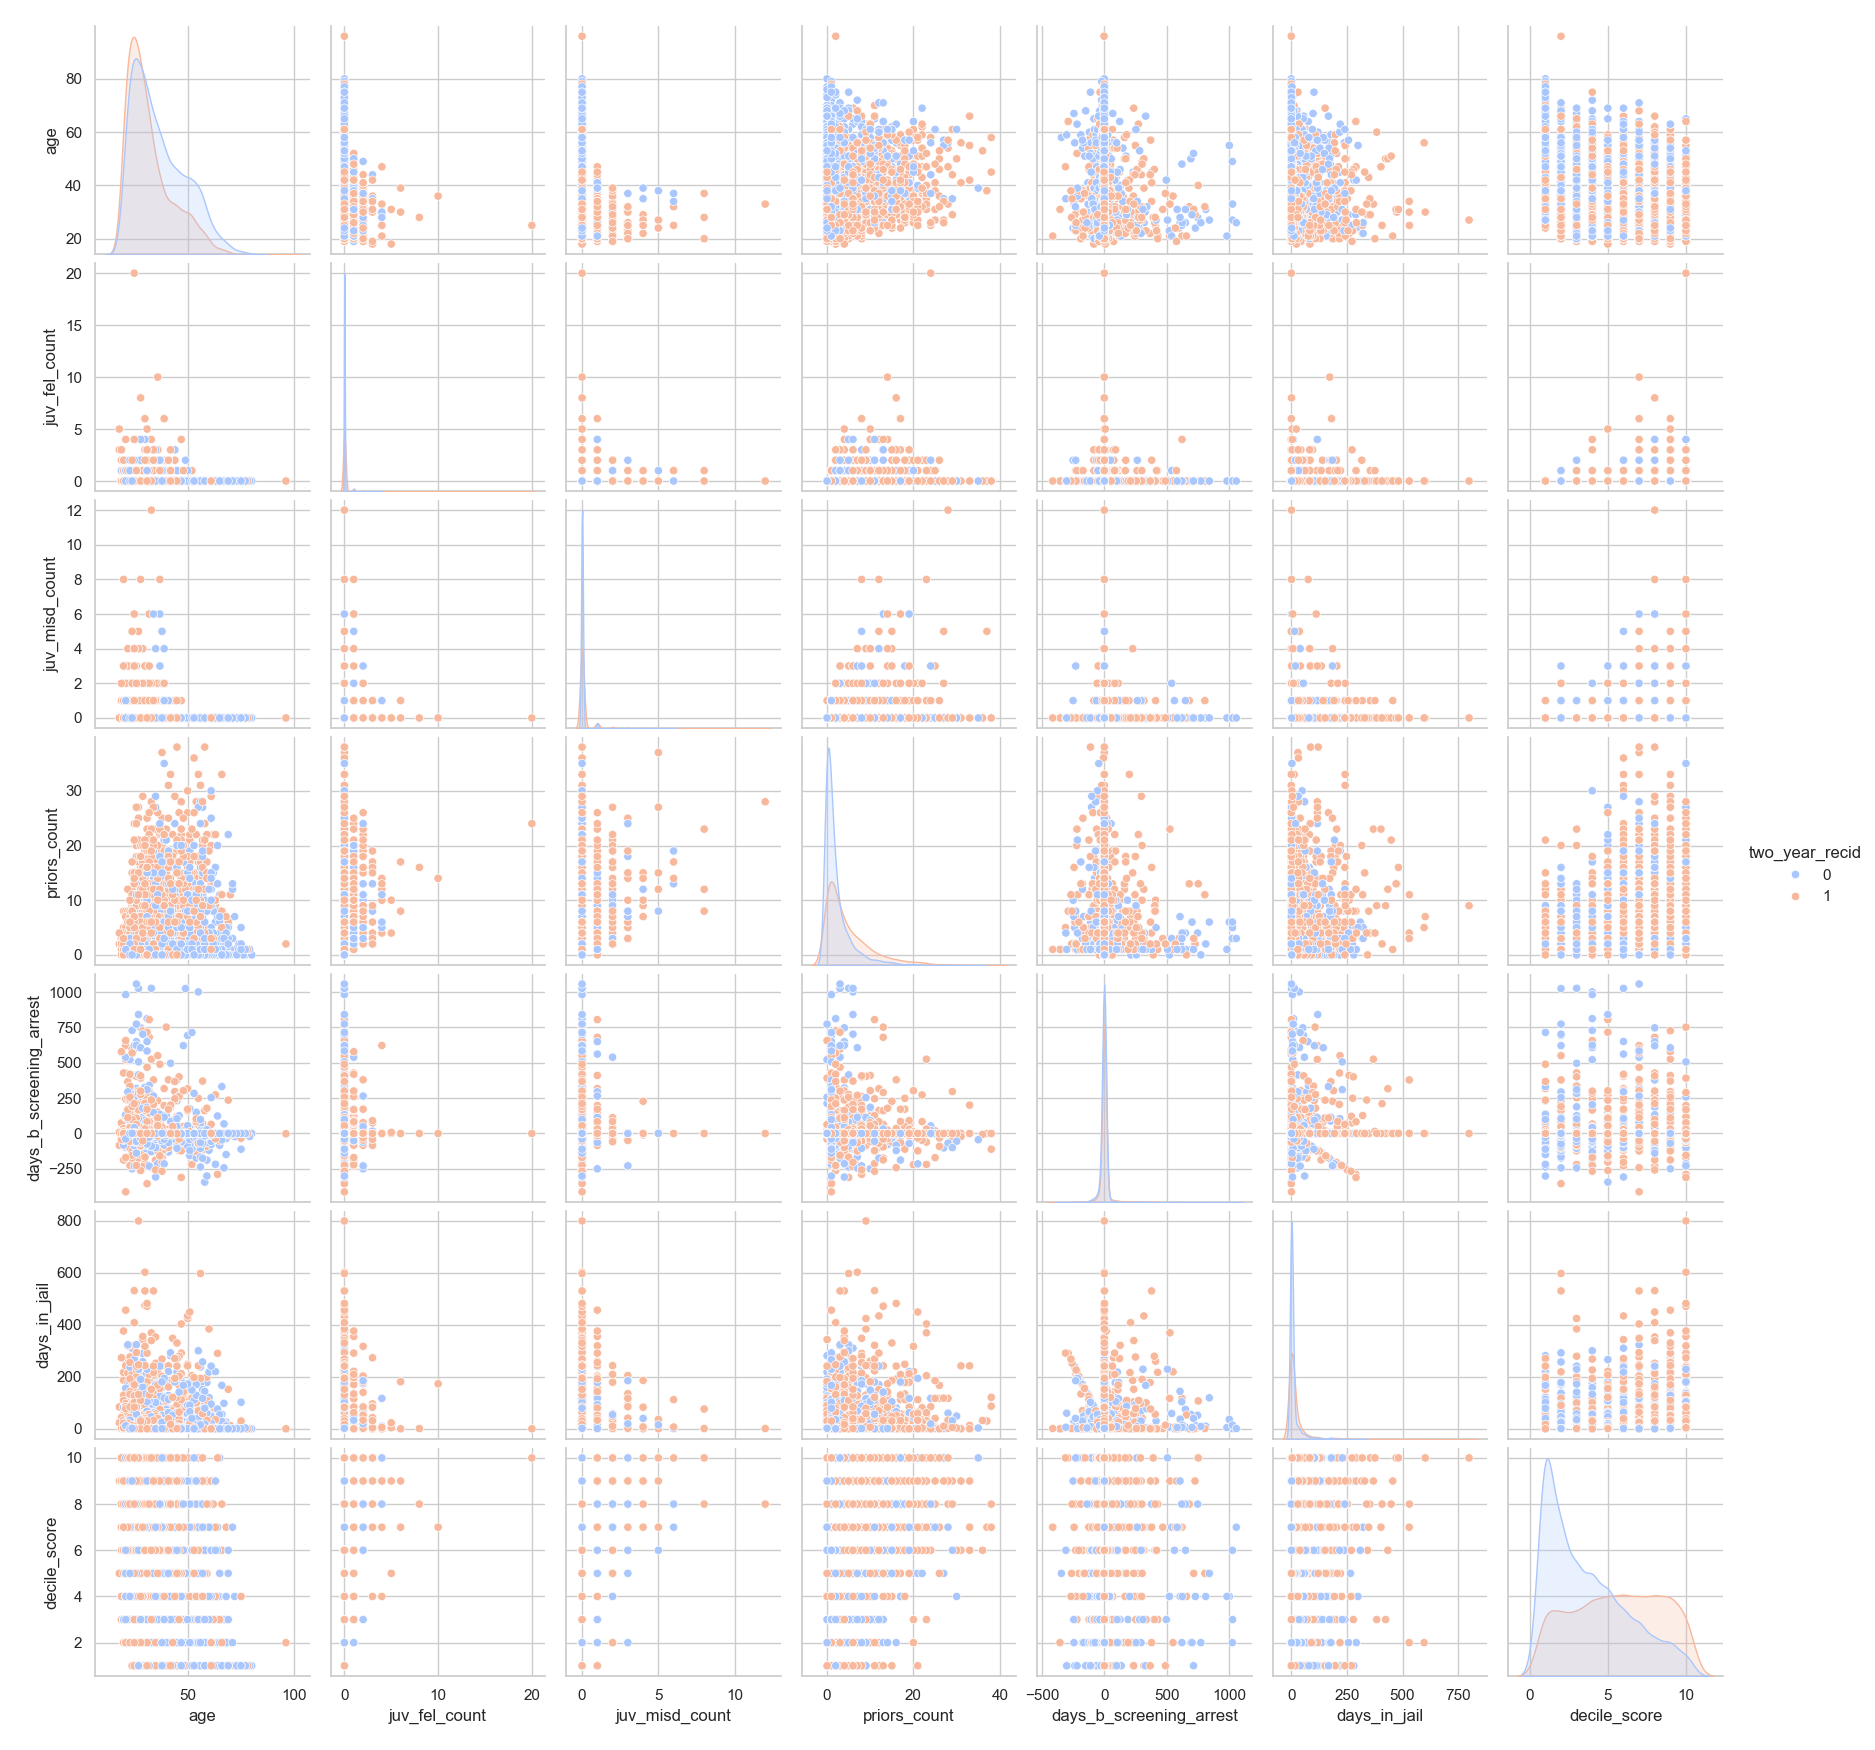
\includegraphics[width=0.7\linewidth]{img/pair_plot}
	\caption{}
	\label{fig:pairplot}
\end{figure}


\begin{itemize}
	\item \textbf{\texttt{age}} vs \textbf{\texttt{priors\_count}}. Younger individuals tend to have fewer prior offences, but the prior count is scattered as age increases, showing that younger offenders tend to continue having problems with the judicial system.
	
	\item \textbf{\texttt{age}} vs \textbf{\texttt{decile\_score}}. Older individuals tend to have lower decile scores. Younger individuals are associated with higher scores.
	
	\item \textbf{\texttt{priors\_count}} vs \textbf{\texttt{decile\_score}}. Positive trend: Higher priors count leads to higher decile scores, suggesting a strong correlation, indicating the tendency for offenders to be viewed as a risk community    
	
	\item The distribution of \textbf{\texttt{decile\_score}}. Two-year recidivists tend to cluster at higher decile scores (6–10 range). Non-recidivists are spread more evenly across scores.        
\end{itemize}



\subsection{Analysis of decile score relationship with race}

The COMPAS dataset has been extensively discussed in recent years regarding the fairness of the scores assigned to individuals, especially considering the race component. Although the tool does not use race as one of the features in decile score prediction, there are concerns that race can be associated indirectly with other features. In this section, we will look at the data from the race point of view to see what patterns we can deduce from the dataset.

As a first step, we create a boxplot to compare the distribution of \textbf{\texttt{decile\_score}} across different racial groups. 

\begin{figure}
	\centering
	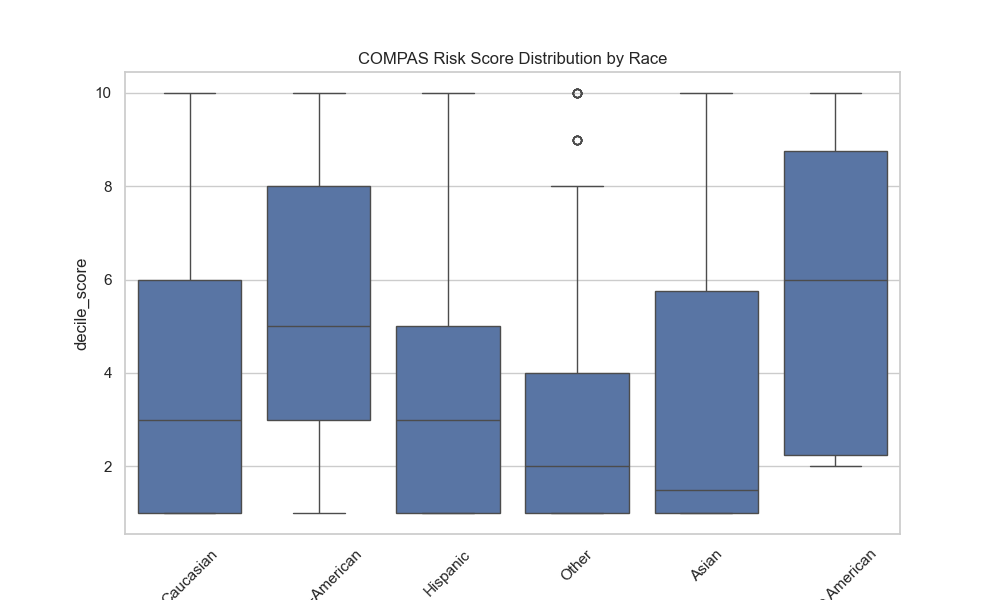
\includegraphics[width=0.7\linewidth]{img/decile_score_by_race_boxplot}
	\caption{}
	\label{fig:decilescorebyraceboxplot}
\end{figure}


From this plot, we notice that African Americans have higher median scores and broader distributions, which suggests a potential bias in the COMPAS scoring system. In addition, Hispanics, Asians, and Other groups scored lower on average, which may indicate differences in the risk assessment process or underlying data inputs.


We then investigated the correlation of \textbf{\texttt{decile\_score}} with \textbf{\texttt{two\_year\_recid}} by race:

\begin{figure}
	\centering
	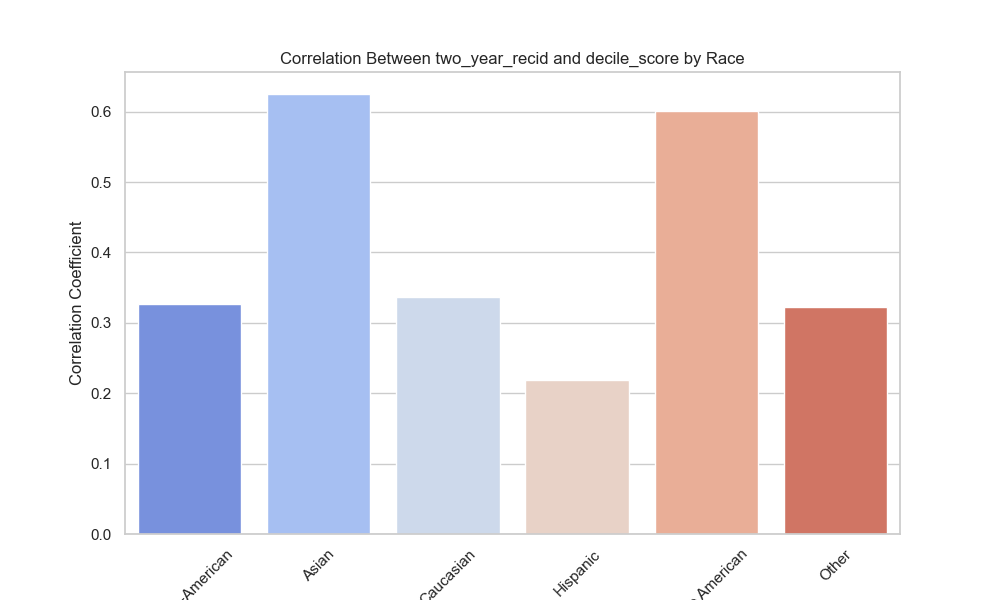
\includegraphics[width=0.9\linewidth]{img/correlation_by_race}
	\caption{}
	\label{fig:correlationbyrace}
\end{figure}

\begin{itemize}
	\item Asians and Native Americans show the highest correlations, indicating that, for these groups, COMPAS scores align more closely with observed recidivism outcomes. However, it is important to remember that these groups comprise a tiny percentage of the population.
	
	\item African-Americans, Caucasians, and Others have moderate correlations, so COMPAS scores are somewhat predictive for these groups but not as strongly as for Asians or Native Americans.
	
	\item The correlation between \textbf{\texttt{two\_year\_recid}} and \textbf{\texttt{decile\_score}} for Hispanics is 0.22, the lowest among the groups, suggesting that for Hispanic individuals, the COMPAS scores are less predictive of actual recidivism outcomes than other racial groups. The low correlation for the Hispanic group is an area of concern because if the COMPAS scores do not accurately predict recidivism for this ethnicity, this could mean that the scoring system may overestimate or underestimate their actual risk, which could lead to misclassification of individuals, leading to potential unfair treatment, for example, harsher parole conditions, sentencing).
\end{itemize}

The distribution of \textbf{\texttt{decile\_score}} for Hispanic individuals was then compared with that of other racial groups using kernel density plots (KDE). 

\begin{figure}
	\centering
	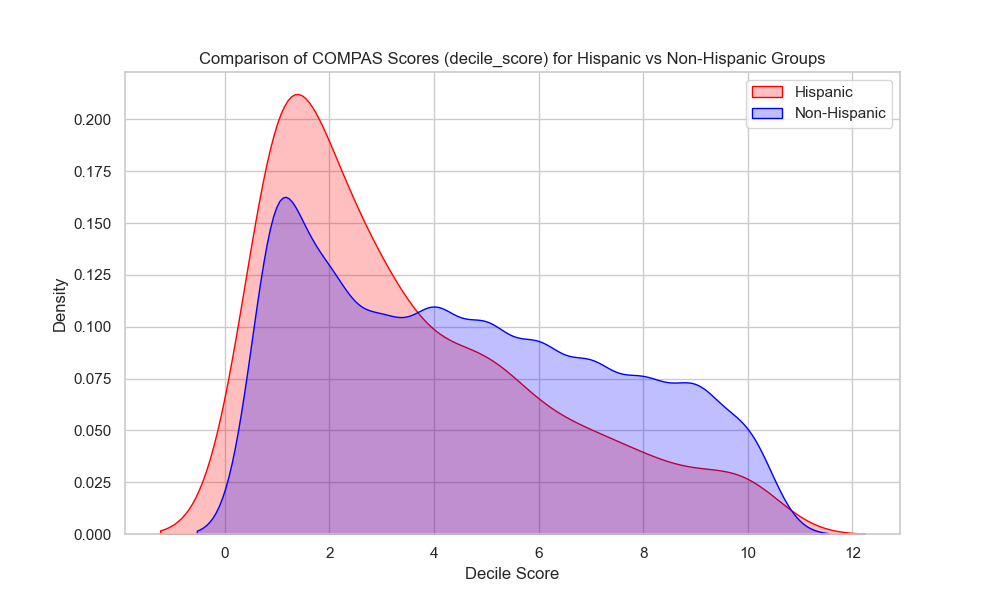
\includegraphics[width=0.7\linewidth]{img/decile_score_by_race_hispanic}
	\caption{}
	\label{fig:decilescorebyracehispanic}
\end{figure}


The plots show that the peak density for Hispanic individuals occurs at a lower score of around 2. In contrast, non-Hispanic individuals have a flatter distribution extending to higher scores, albeit peaking in the same region, suggesting that Hispanic individuals are more likely to receive lower COMPAS scores than non-Hispanic individuals.

One has to note that we have previously seen that Hispanic individuals account for 8.8\% of the population, which is significantly smaller compared to African-American and Caucasian groups.
Although by any means not conclusive, these aspects raise questions about how risk scores are calibrated for underrepresented groups.

\subsubsection{Analysis of the African-American sector}


We created another density plot to compare the distribution of risk scores between African-American individuals and non-African-American individuals.

\begin{figure}
	\centering
	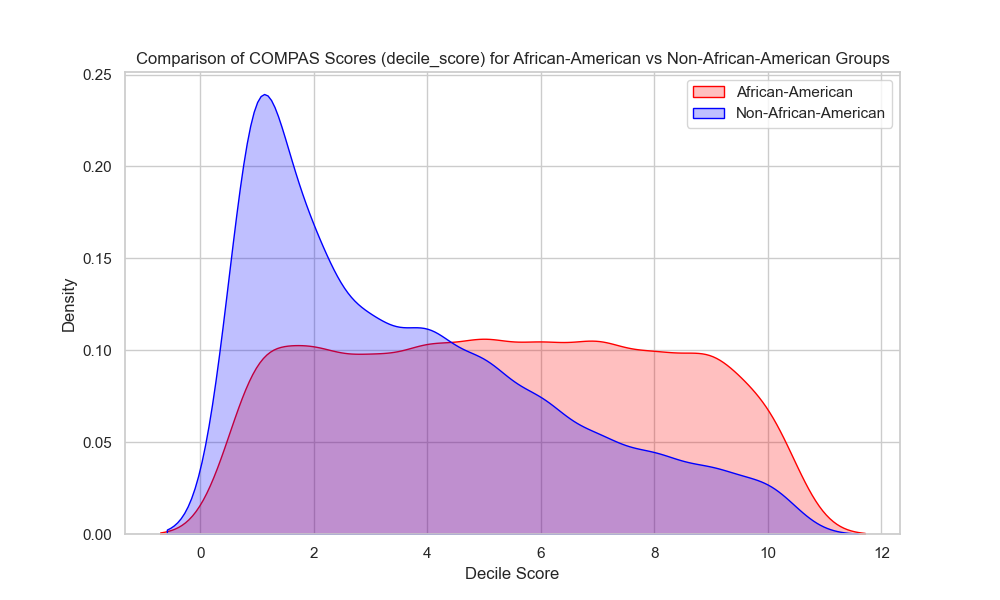
\includegraphics[width=0.7\linewidth]{img/decile_score_by_race_african_american}
	\caption{}
	\label{fig:decilescorebyraceafricanamerican}
\end{figure}


Here, we notice that African Americans are more likely to receive risk scores in the higher decile range, exceeding a value of six, than non-African Americans, suggesting that the COMPAS tool systematically assigns higher risk scores to African Americans. As noticed previously, non-African-American individuals show a strong peak at around a score of 2, with fewer individuals in this group receiving scores in the higher ranges.

This disparity in score distributions raises concerns about potential bias in the COMPAS scoring system. African Americans appear to be disproportionately classified as higher risk, a factor which could impact downstream decisions such as sentencing or parole.

\subsection{Robustness of \textbf{\texttt{decile\_score}}}

As a final analysis, we compare \textbf{\texttt{decile\_score}} with \textbf{\texttt{two\_year\_recid}} to see how many high-risk individuals receded and how many individuals categorised as low-risk did not. This metric is very powerful, as it assesses the validity of the predicted risk metric. Throughout this study, we will also use this test to validate our predicted scores for the machine learning models.


An important decision in this exercise is the selection of the decile score threshold that will dictate that values above it are more likely to recidivate and those below it not. In order to do this, we compared the decile score and two-year record for multiple thresholds. We examined the number of true negatives (the individuals with a decile score lower than the threshold and did not recidivate), true positives (those with a decile score higher or equal than the threshold and did recidivate) and false positives and negatives. We then used these results to calculate the sensitivity, specificity, precision and accuracy:

\begin{table}[h!]
	\centering
	\begin{tabular}{|c|c|c|c|c|}
		\hline
		\textbf{Threshold} & \textbf{Sensitivity} & \textbf{Specificity} & \textbf{Precision} & \textbf{Accuracy} \\ \hline
		4                               & 0.628659             & 0.670551             & 0.60941            & 0.651707          \\ \hline
		5                               & 0.521186             & 0.766299             & 0.645823           & 0.656039          \\ \hline
		6                               & 0.411017             & 0.83811              & 0.674889           & 0.645989          \\ \hline
		7                               & 0.3047               & 0.897323             & 0.708147           & 0.63074           \\ \hline
		8                               & 0.196071             & 0.938268             & 0.721986           & 0.604401          \\ \hline
	\end{tabular}
	\caption{Performance Metrics for Different Decile Score Thresholds}
	\label{tab:performance_metrics}
\end{table}

Following this procedure, a threshold of 5 was decided to provide the best balance of these metrics. With this threshold, the total accuracy and precision are moderate, indicating that while the model performs reasonably well overall, there is room for improvement. We notice a low sensitivity compared to specificity; the model is better at identifying non-recidivists than recidivists.


The metrics for each racial group were then calculated with this threshold.


The Caucasian group has a relatively high specificity but low sensitivity, indicating the COMPAS model more effectively avoids false positives but struggles to identify true positives. 

The African-American group shows higher sensitivity but lower specificity compared to Caucasians. This suggests the model identifies more recidivists among African Americans but at the cost of more false positives.


The Hispanic group has low sensitivity, meaning the model struggles significantly to identify true positives in this group. Precision is also the lowest, indicating a high false-positive rate.


The significant disparity in sensitivity and specificity across racial groups highlights potential fairness issues in the model's predictions. For example, the model disproportionately favours Caucasians and Asians in terms of specificity while penalizing African-Americans with higher false-positive rates.




%pipeline
%--------


\subsection{Preparing data for machine learning}

	Building on the insights derived from the previous section, the next step involved the creation of the pipeline to transform the raw dataset into a format optimized for machine learning models.
	
	\begin{figure}[H]
		\centering
		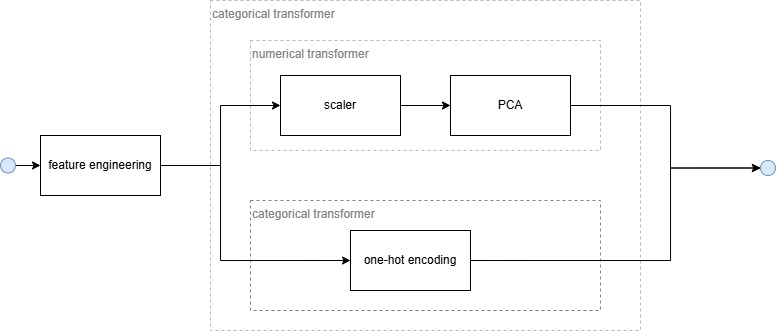
\includegraphics[width=0.7\linewidth]{img/pipeline}
		\caption{}
		\label{fig:pipeline}
	\end{figure}
	
	The pipeline created for this application is shown in Figure \ref{fig:pipeline}. It is based on the \texttt{Pipeline} functionality provided by the Scikit-learn library, integrating feature engineering and transformations for both numerical and categorical data. The pipeline consists of the following components:

	\begin{itemize}
		\item \textbf{Feature Engineering:}
		The pipeline begins with a feature engineering unit where raw features are processed to derive new attributes and filter out irrelevant ones. This step prepares the dataset for subsequent transformations. Feature engineering is based on the Python’s \texttt{pandas} library. The transformation logic was encapsulated in a reusable function, \texttt{feature\_engineering}, which was wrapped in a \texttt{FunctionTransformer} to integrate it into  the machine learning pipeline. 
		
		The primary objective of the feature engineering step is to:
		\begin{itemize}
			\item Retain only the most relevant features for recidivism prediction.
			\item Derive new features to enhance the dataset’s predictive capacity.
			\item Remove unnecessary or redundant columns to reduce noise and complexity.
		\end{itemize}
		
		Following the analysis phase, a subset of the dataset's features was identified as relevant for training and subsequent analysis. These include demographic attributes (e.g., \texttt{age}, \texttt{race}, \texttt{sex}), prior criminal history (\texttt{priors\_count}), juvenile offense counts (\texttt{juv\_fel\_count}, \texttt{juv\_misd\_count}, \texttt{juv\_other\_count}), and timestamps related to jail custody (\texttt{c\_jail\_in}, \texttt{c\_jail\_out}) and general custody (\texttt{in\_custody}, \texttt{out\_custody}). Features such as names and IDs were excluded to avoid introducing irrelevant or sensitive information into the analysis.
		
		We decided to keep the \texttt{race} feature so that we can use it to analyse the results obtained by the machine learning models, but it will be removed from the features set at a later stage.
		
		Two new features were created to capture time-based patterns:
		\begin{itemize}
			\item \textbf{\texttt{days\_in\_jail}}: Calculated as the absolute difference in days between the \texttt{c\_jail\_in} and \texttt{c\_jail\_out} timestamps. This feature provides insight into the duration of incarceration for a given charge.
			\item \textbf{\texttt{days\_in\_custody}}: Calculated as the absolute difference in days between the \texttt{in\_custody} and \texttt{out\_custody} timestamps. This feature reflects the total time an individual spent in custody.
		\end{itemize}
		
		These features offer information about the extent of an individual’s interaction with the criminal justice system, which may correlate with recidivism likelihood. As the originating features  had frequent nulls, zeros were imputed where the calculation did not result into a number.
		
		The final processed dataset contains the following columns:
		\begin{itemize}
			\item \textbf{Demographic Features}: \texttt{sex}, \texttt{age}, \texttt{race}.
			\item \textbf{Juvenile Offense Counts}: \texttt{juv\_fel\_count}, \texttt{juv\_misd\_count}, \texttt{juv\_other\_count}.
			\item \textbf{Criminal History}: \texttt{priors\_count}.
			\item \textbf{Derived Features}: \texttt{days\_in\_jail}, \texttt{days\_in\_custody}.
		\end{itemize}
		
		This feature engineering process resulted in a clean and concise dataset, ready for use in machine learning pipelines. By deriving meaningful features and eliminating irrelevant data, the preprocessing step set a strong foundation for building predictive models.
		
		
		\item \textbf{Numerical transformer:}
		\begin{itemize}
			\item \textbf{Scaler:} Numerical features are standardized or normalized to ensure they are on a similar scale. This step is critical for distance-based algorithms and gradient-based optimization.
			\item \textbf{PCA (Principal Component Analysis):} After scaling, dimensionality reduction is applied to numerical features to eliminate redundancy and reduce the complexity of the data. PCA retains the most important components that explain the majority of variance in the data.
		\end{itemize}
		
		\item \textbf{Categorical Transformer:}
		\begin{itemize}
			\item \textbf{One-Hot Encoding:} Categorical variables are transformed into numerical format using one-hot encoding. This technique creates binary columns for each category, ensuring compatibility with machine learning models.
		\end{itemize}
		
		\item \textbf{Integration of Transformations:}
		The outputs from the \textit{numerical transformer} and \textit{categorical transformer} are combined into a unified dataset using the Scikit-learn pipeline framework. This ensures that the transformations are consistently applied to both training and testing datasets, improving reproducibility and minimizing data leakage.
	\end{itemize}
	
	This pipeline structure allows for the independent processing of numerical and categorical features, enabling specialized transformations for each type of data. The modular design, powered by Scikit-learn’s \texttt{Pipeline} and \texttt{ColumnTransformer}, ensures flexibility and reusability, making it adaptable to various datasets and machine learning workflows. By incorporating scaling, PCA, and encoding, the pipeline ensures the dataset is well-prepared, reducing potential biases or inefficiencies during model training.
	
	This approach represents an effective preprocessing strategy for heterogeneous datasets and highlights the importance of tailored transformations for achieving robust model performance.
	
	\section{Experiments}
	
	We start this investigation by explaining very shortly the project structure for this exercise. Unlike analysis, Python files were used to create the models, tune them and carry out experiments. 
	
	
	\begin{itemize}
		\item A \textbf{utils} area contains all the scripts necessary to download the dataset, split it in train and test datasets, define the feature engineering module and create the preprocessing pipeline. As most of these scripts manipulate the dataset, their result is ultimately saved in a \textbf{data} folder.
		
		\item A \textbf{models} area contains the definition of the k-nearest neighbour, logistic regressor and neural network. In all three model definitions, an initial step is to try and access a 'best parameters' file that contains the result of an optimization step that is described later on in this list. The model is combined with the preprocessor  to create the model pipeline.
		
		\item An \textbf{experiments} area contains all the experiments that are carried out as part of this exercise. It contains three types of modules:
		
		\begin{enumerate}
			\item A script is designed to evaluate the performance of a machine learning pipeline on test data. It computes and reports key metrics, including accuracy, ROC AUC, F1-scores for both classes, precision, overall accuracy, and weighted average F1. The evaluation includes generating and saving a classification report, a confusion matrix visualization, and an ROC curve plot. Results are saved in \textbf{results} folder for further analysis.
			
			\item \textbf{Experiment} scripts for each of the three machine learning methods that is used for training, evaluating, and saving a model pipeline. It loads the training and test datasets, fits the specified model pipeline on the training data, evaluates its performance on the test data using the functions explain previously, and saves the trained pipeline to a file for future use.
			
			\item \textbf{Optimization} scripts that tune our machine learning model pipelines using grid search with cross-validation. After completing the grid search, each script identifies and saves the best parameters and corresponding cross-validation accuracy. It also exports the full results of the grid search as a CSV file for detailed analysis. This process ensures a systematic and reproducible approach to selecting optimal model hyperparameters.
		\end{enumerate}
	\end{itemize}
	
	
	\bigskip
	\subsubsection{Logistic regression experiments}
	
	Logistic regression results demonstrate that the model achieved a test accuracy of approximately 69.5\%, and a ROC AUC of 0.74 as can be seen in Figure \ref{fig:logisticregressionroc}, outperforming the baseline COMPAS results in several key areas. The logistic regression model demonstrated better overall accuracy compared to COMPAS and a higher ROC AUC, indicating improved discriminatory power in separating the two classes. Furthermore, the F1-score for the minority class was significantly higher, reflecting a better balance between precision and recall, particularly for the harder-to-predict positive class.
	
	Examining the confusion matrix show in Figure \ref{fig:logisticregressioncm} further illustrates the logistic regression model's improvements. The tuned model identified fewer false positives and false negatives relative to the COMPAS predictions, suggesting that logistic regression was more effective at minimizing classification errors across both classes. The tuned model demonstrated better precision and recall for class 1, likely due to its capacity for optimization during the tuning phase, whereas COMPAS appears to struggle more with recall, as evidenced by its larger number of false negatives. This is a significant improvement as false negatives correspond to the people that has a high decile score but did not have further encounters with the legal system.
	
	\begin{figure}[H]
		\centering
		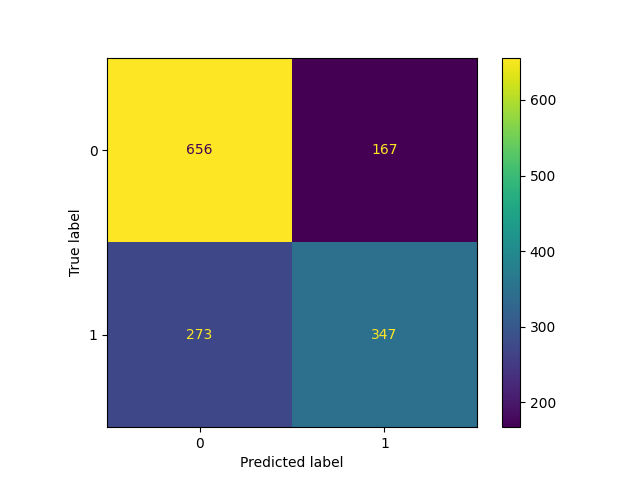
\includegraphics[width=0.7\linewidth]{img/logistic_regression_cm}
		\caption{Confusion matrix for logistic regression model}
		\label{fig:logisticregressioncm}
	\end{figure}
	
	\begin{figure}[H]
		\centering
		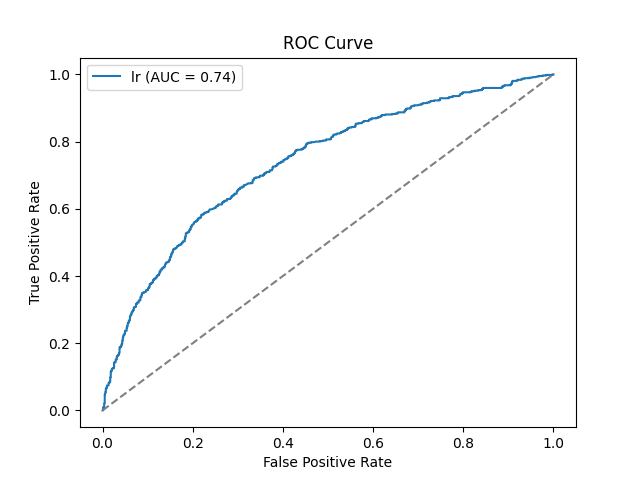
\includegraphics[width=0.7\linewidth]{img/logistic_regression_roc}
		\caption{Receiver operator characteristic plot for logistic regression model}
		\label{fig:logisticregressionroc}
	\end{figure}
	
	
	The \texttt{class\_weight='balanced'} parameter in Scikit-learn's \texttt{LogisticRegression} adjusts the weights of the classes inversely proportional to their frequencies in the training data, effectively addressing class imbalance. By assigning higher importance to the minority class 1, this parameter ensures that the model does not disproportionately favor the majority class 0. As a result, the recall for class 1 improved to 0.67 compared to previous configurations, indicating that the model is better at correctly identifying instances of the minority class. However, this improvement came at a slight cost to precision for both classes, as the model now predicts class 1 more frequently, leading to a lower overall accuracy (67.71\%). 
	
	With the balanced weights, the model's improved recall for the minority class, that individuals who will reoffend,  may lead to better proactive interventions. However, the trade-off is an increase in false positives, which could mean incorrectly labelling individuals as high risk. This could unfairly subject some individuals to harsher penalties
	
	This result highlights the ethical and societal implications of optimizing machine learning models, especially for imbalanced datasets.
	
	
	
	\bigskip
	\subsubsection{K-nearest neighbour experiments}
	
	The k-Nearest Neighbors (kNN) model achieved a test accuracy of 73.46\% and a ROC AUC of 0.80 as can be seen in Figure \ref{fig:knnroc}, which are notable improvements over the COMPAS results and slightly better than the logistic regression model. The precision and recall metrics for class 1 are 0.73 and 0.60, respectively, resulting in an F1-score of 0.66. This performance demonstrates that kNN is more effective at balancing the prediction of both classes, with a better trade-off between precision and recall compared to logistic regression and COMPAS. The ROC AUC score of 0.8 highlights the model’s strong ability to differentiate between the two classes.
	
	Compared to logistic regression, the confusion matrix for kNN, shown in Figure \ref{fig:knncm} shows fewer false positives and a higher number of true positives. This suggests that kNN is better at minimizing classification errors for the majority class while still improving recall for the minority class. Compared to COMPAS, kNN drastically reduces false negatives and false positives, making it a significantly more balanced and fair model for this classification task.
	
	In practical terms, the improved performance of kNN translates to more accurate predictions, particularly for identifying individuals at higher risk. This could lead to better decision-making, reducing the likelihood of unfairly labeling low-risk individuals as high risk while improving the identification of true high-risk cases. 	
	
	
	\begin{figure}[H]
		\centering
		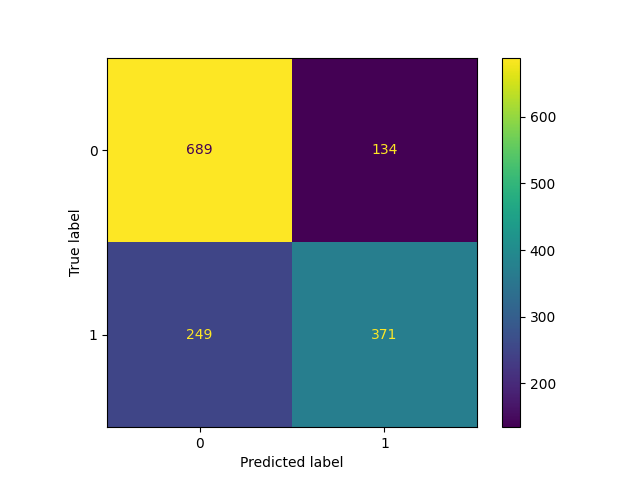
\includegraphics[width=0.7\linewidth]{img/knn_cm}
		\caption{Confusion matrix for k-nearest neighbour model}
		\label{fig:knncm}
	\end{figure}
	
	\begin{figure}[H]
		\centering
		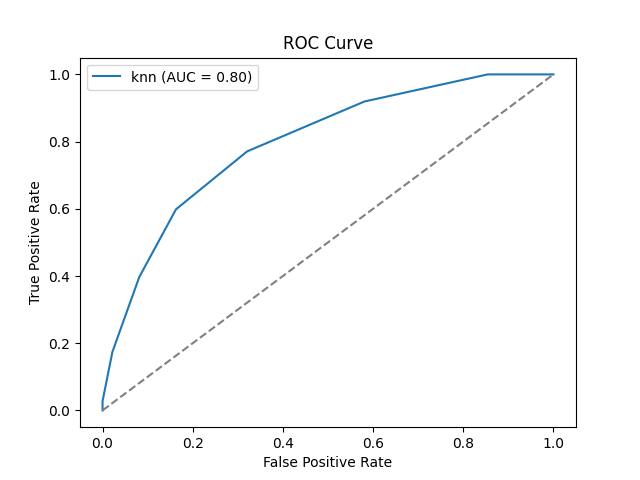
\includegraphics[width=0.7\linewidth]{img/knn_roc}
		\caption{Receiver operator characteristic plot for k-nearest neighbour model}
		\label{fig:knnroc}
	\end{figure}
	
	
	
	The k-Nearest Neighbors (kNN) model configured with \texttt{weights='distance'} demonstrated exceptional performance, achieving a test accuracy of 98\% and a near-perfect ROC AUC score of 0.9991 as can be seen in Figure \ref{fig:knnrocdistance}. By weighting closer neighbors more heavily, the model effectively used local information to make better predictions. According to the classification report, the model achieved a precision of 0.97, recall of 1.00, and F1-score of 0.98 for class 0, and a precision of 1.00, recall of 0.95, and F1-score of 0.98 for class 1. This indicates balanced and superior performance across both classes. As can be seen in Figure \ref{fig:knncmdistance}, the confusion matrix further highlights this improvement, with only 30 misclassified instances.
	
	While these results are remarkable, they also raise important ethical considerations. The dramatic improvement in performance suggests that the model may be overfitting to the training data, particularly since the dataset is relatively small and lacks variability. The use of \texttt{weights='distance'} could amplify biases present in the dataset, as the model prioritizes local data points, which may inadvertently reflect systemic or historical inequalities. In applications such as recidivism prediction, this could lead to overly confident predictions that disproportionately impact certain groups, raising concerns about fairness and accountability. Thus, while the improved performance is promising, careful validation on diverse and representative datasets is necessary to ensure the model's robustness and equitable application.
	
	\begin{figure}[H]
		\centering
		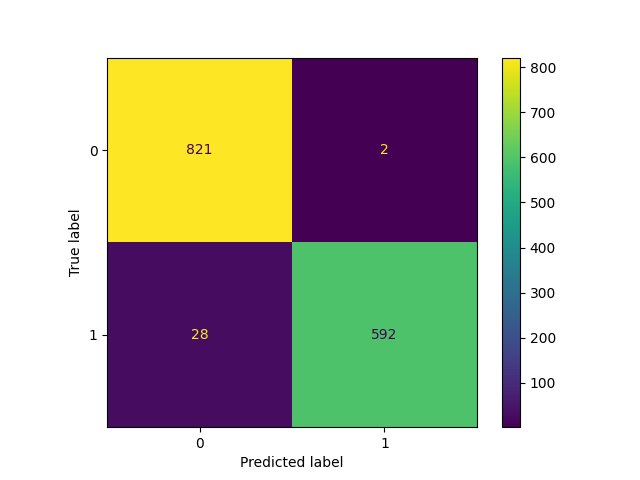
\includegraphics[width=0.7\linewidth]{img/knn_cm_distance}
		\caption{Confusion matrix for k-nearest neighbour model with weights parameter set to distance. This is probably the result of overfitting.}
		\label{fig:knncmdistance}
	\end{figure}
	
	\begin{figure}[H]
		\centering
		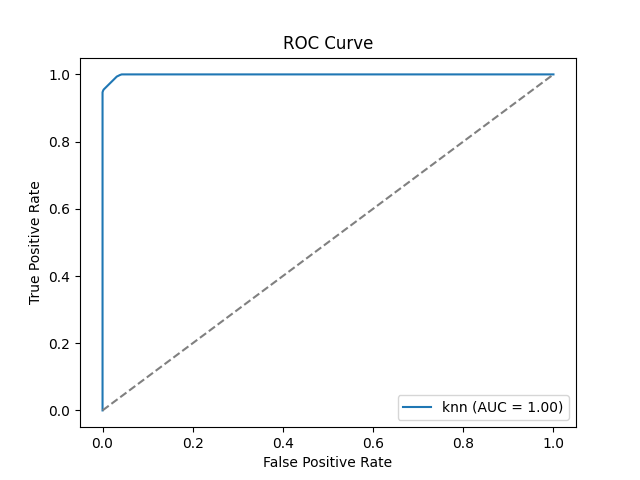
\includegraphics[width=0.7\linewidth]{img/knn_roc_distance}
		\caption{Receiver operator characteristic plot for k-nearest neighbour model with weights parameter set to distance. This is probably the result of overfitting.}
		\label{fig:knnrocdistance}
	\end{figure}
	
	
	\bigskip
	\subsubsection{Neural network experiments}
	
	The neural network implemented in exercise consists of an input layer, followed by two fully connected hidden layers. The first hidden layer contains 128 neurons, and the second contains 64 neurons, each followed by batch normalization and a ReLU activation function. The output layer consists of 2 neurons with a softmax activation function. The model is trained using the cross-entropy loss function, optimized with the Adam optimizer, and employs a mini-batch training strategy with a default batch size of 32 and 20 epochs.
	
	
	The neural network achieved a test accuracy of 70\% and a ROC AUC score of 0.75, reflecting moderate performance in distinguishing between the two classes. The model attained a precision of 0.75, recall of 0.71, and F1-score of 0.73 for class 0, while for class 1, the precision was 0.64, recall was 0.69, and F1-score was 0.66. These metrics highlight that the model performs slightly better for the majority class but still maintains a balanced recall across both classes, which is important in scenarios like this with potential imbalance. The confusion matrix shows 242 false positives and 191 false negatives, indicating that while the model correctly predicts most instances, there is room for improvement.
	
	
		\begin{figure}[H]
		\centering
		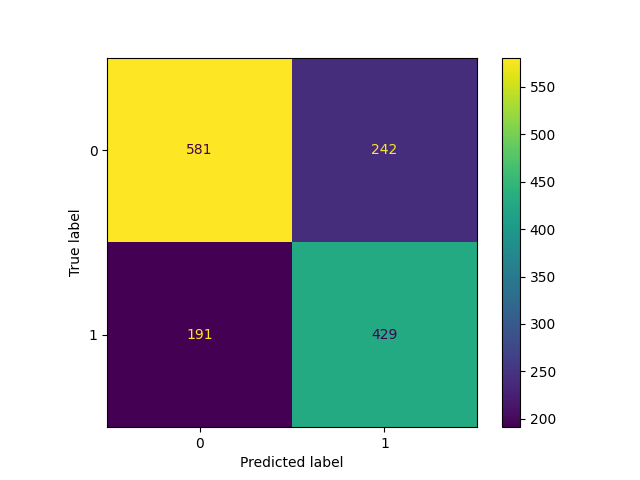
\includegraphics[width=0.7\linewidth]{img/nn_cm}
		\caption{Confusion matrix for neural network model.}
		\label{fig:nncm}
	\end{figure}
	
	\begin{figure}[H]
		\centering
		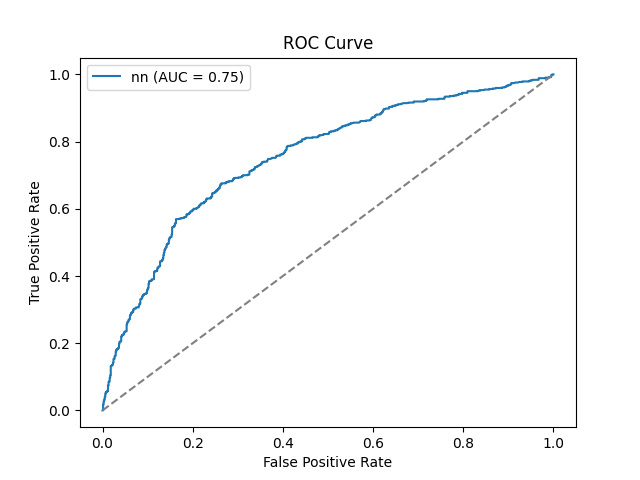
\includegraphics[width=0.7\linewidth]{img/nn_roc}
		\caption{Receiver operator characteristic plot for neural network model.}
		\label{fig:nnroc}
	\end{figure}
	
	
	Changing the loss function to mean squared error caused some differences in how the network performs. While the overall accuracy stayed the same, the model became better at identifying instances of the minority class but less precise when predicting the majority class. This happened because MSE treats errors more evenly, which helps the model focus on reducing overall mistakes rather than just making the most confident predictions.
	
	By using MSE, the model seems to make fairer predictions across both classes, improving recall for the minority class. However, this comes with a trade-off: the model may not be as confident in its predictions. Choosing MSE or another loss function depends on what matters most for the task—whether it's catching as many minority cases as possible or making highly confident predictions.
	
	\subsubsection{Final comments on experiments}
	

	
	Table \ref{tab:metrics} summarizes the performance metrics across the different techniques. Logistic regression (\texttt{lr}) and its class-weighted variant (\texttt{lr balanced}) provide baseline results, with the balanced variant slightly improving recall for the minority class but at the cost of precision and overall accuracy. The weighted F1-score also slightly decreased, reflecting the trade-off in class predictions.
	
		
	\begin{table}[H]
		\centering
		\begin{tabular}{|l|c|c|c|c|}
			\hline
			\textbf{Technique} & 
			\makecell{F1-Score \\Class 0\\Class 1} & 
			\makecell{Precision \\ (Class 1)} & 
			\makecell{Overall\\Accuracy} & 
			\makecell{Weighted\\Avg\\F1-Score} \\ \hline
			lr & \makecell { 0.75 \\ 0.61 } & 0.68 & 0.70 & 0.68 \\ \hline
			lr balanced & \makecell { 0.71 \\ 0.64 } & 0.61 & 0.68 & 0.67 \\ \hline
			knn & \makecell { 0.78 \\ 0.66 } & 0.73 & 0.73 & 0.72 \\ \hline
			knn distance & \makecell { 0.98 \\ 0.98 } & 1.00 & 0.98 & 0.98 \\ \hline
			nn & \makecell { 0.76 \\ 0.62 } & 0.66 & 0.70 & 0.69 \\ \hline
			nn mse& \makecell { 0.72 \\ 0.68 } & 0.63 & 0.70 & 0.70 \\ \hline
		\end{tabular}
		\caption{Performance Metrics for Classification Techniques}
		\label{tab:metrics}
	\end{table}
	
	
	
	The k-Nearest Neighbors (\texttt{knn}) model performed better than logistic regression in both overall accuracy and weighted F1-score, with a significant improvement in capturing minority class instances. The use of distance-based weights (\texttt{knn distance}) led to exceptional performance, with near-perfect metrics across all evaluation categories. However, this result might indicate potential overfitting and should be carefully validated on unseen data before drawing conclusions.
	
	The neural network (\texttt{nn}) achieved comparable performance to logistic regression, with a slight improvement in recall for the minority class. Changing the loss function to mean squared error (\texttt{nn mse}) resulted in a better balance between precision and recall for both classes, leading to a slight improvement in the weighted F1-score compared to the cross-entropy loss variant. This suggests that MSE as a loss function can encourage fairer predictions across classes in certain scenarios.
	
	Overall, \texttt{knn} outperformed \texttt{lr} and \texttt{nn} models in most metrics, with \texttt{nn mse} demonstrating improved balance compared to \texttt{nn}. However, the extremely high metrics of \texttt{knn distance} should be interpreted with caution, as they may not generalize well to unseen data. The choice of model and loss function should depend on the specific application and the importance of precision, recall, and generalization.
	
	
	\subsection{Ethical Review}
		
	The analysis of the data, model performance, and insights generated raises several ethical concerns and societal implications that warrant careful evaluation. First, the dataset used for training likely reflects inherent biases from historical or systemic inequalities, particularly in domains such as recidivism prediction. If the dataset is biased, models trained on it, regardless of their performance metrics, may inadvertently perpetuate or amplify these biases. For instance, minority groups may face disproportionately higher false positive or false negative rates, which could lead to unjust outcomes such as harsher treatment or denied opportunities.
	
	The insights generated by these models also need to be critically examined. While models like \texttt{knn distance} demonstrated near-perfect performance on the test set, such high metrics often indicate overfitting, meaning the model may not generalize well to new or unseen data. Overfitting, combined with biased data, could result in overly confident predictions that fail to account for the complexities of real-world cases. This raises questions about the trustworthiness of these insights, especially in high-stakes decisions that affect individuals' lives.
	
	From a societal perspective, the implications of deploying these models are profound. A model with high false positive rates for the minority class (e.g., labeling individuals as high risk when they are not) can lead to unfair treatment, reinforcing discrimination and systemic inequities. Conversely, high false negative rates (e.g., failing to identify high-risk individuals) could pose public safety concerns. These outcomes highlight the importance of balancing precision and recall while ensuring fairness and transparency in predictions.
	
	To mitigate these ethical risks, several measures are necessary. Regular bias audits should be conducted on the dataset and model outputs to identify and address disparities. Additionally, stakeholders must be involved in the development process to ensure that the models align with societal values and legal standards. Explainability techniques should also be employed to make model predictions more interpretable, allowing decision-makers to understand the rationale behind predictions. Finally, models should be rigorously tested on diverse and representative datasets to ensure robustness and fairness across different demographic groups.
	
	In summary, while the results demonstrate strong technical performance, the ethical considerations of bias, fairness, and societal impact must remain at the forefront. Developing and deploying machine learning models in sensitive domains requires a careful balance between accuracy and equity, with continuous efforts to ensure accountability and mitigate harm.
	
	
	
	


	


	
	
	
	
	
	
	
	

	
	



